\documentclass[10pt,twocolumn]{scrartcl}
\usepackage[a4paper,width=170mm,top=25mm,bottom=25mm,bindingoffset=3mm]{geometry}
\setlength{\parskip}{1em}

\usepackage{lipsum}
\usepackage[pdftex]{graphicx} 
\usepackage{url} 
\usepackage{lipsum} 
\usepackage{float}
\usepackage{amsmath}
\usepackage{subcaption}
\usepackage{mwe}
\usepackage{multicol}

\renewenvironment{abstract}
 {\quotation\large\noindent\rule{\linewidth}{.5pt}\par\smallskip
  {\centering\bfseries\abstractname\par}\medskip}
 {\par\noindent\rule{\linewidth}{.5pt}\endquotation}

\begin{document}

\renewcommand{\refname}{References}
\begin{titlepage}

\begin{center}


\includegraphics[width=0.25\textwidth]{img/collegecrest.png}\\
\vspace{3em}

\Huge\textbf{Our project}\\
\vspace{1em}
{\normalsize {\textbf Group 1}\\}
 \vspace{1em}
{\Large{\textbf Department of Bioengineering \\ Imperial College London}}\\[0.5in]

{\large\emph{A Project Report Submitted in \\Partial Fulfilment of the\\ MEng ----- Degree}}
\vspace{1in}

      
\normalsize {\textbf Supervisor:} \\
Supervisor Name\\
\vspace{1em}
Department of your Supervisor \\
% \vspace{1em}
\url{supervisor@ic.ac.uk}
\vfill
June, 2022
\end{center}
\end{titlepage}
 

\twocolumn[
\begin{@twocolumnfalse}
	\title{Your Project Title Here}
\author{Your Names Here}
\maketitle

\begin{abstract}
Lorem ipsum dolor sit amet, consectetuer adipiscingelit. Ut purus elit, vestibulum ut, placerat ac, adipisc-ing vitae, felis. Curabitur dictum gravida mauris. Namarcu libero, nonummy eget, consectetuer id, vulputatea, magna.  Donec vehicula augue eu neque.  Pellen-tesque habitant morbi tristique senectus et netus etmalesuada fames ac turpis egestas. Mauris ut leo. Crasviverra metus rhoncus sem.  Nulla et lectus vestibu-lum urna fringilla ultrices. Phasellus eu tellus sit amettortor gravida placerat. Integer sapien est, iaculis in,pretium quis, viverra ac, nunc. Praesent eget sem velleo ultrices bibendum.  Aenean faucibus.  Morbi do-lor nulla, malesuada eu, pulvinar at, mollis ac, nulla.Curabitur auctor semper nulla. Donec varius orci egetrisus.  Duis nibh mi, congue eu, accumsan eleifend,sagittis quis, diam. Duis eget orci sit amet orci dignis-sim rutrum.
\end{abstract}
\end{@twocolumnfalse}]

\section{Introduction}
\subsection{Project Overview}
The purpose of this project is to check that the PCB board of ePATH functions properly. This would help ensure that it was properly manufactured by the factory and it will help smooth identification of faults during maintenance. The process must be automated and user-friendly to enable any technician without good knowledge of the electronics of ePATH perform this test. A


\begin{figure}[H]
          \centering
          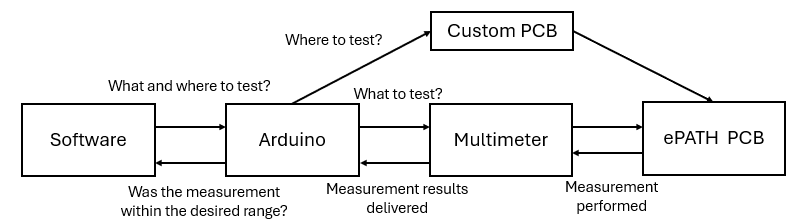
\includegraphics[width=1\linewidth]{img/General end goal diagram.png}
          \caption{Image 1}
          \label{fig:1}
    \end{figure}

\subsection{Main Objective}
The specific objectives of the project were: 
\begin{itemize}
\item 
\item To ...... 
\item To ...............
\end{itemize}

\subsection{Extra section}
\lipsum[1] 
\section{Background}

\subsection{Subtopic}
\lipsum[1]

\noindent If you want to add an image, you can do it like this:

\begin{figure}[H]
          \centering
          
\includegraphics[width=1\linewidth]{img/bioeng.jpg}
          \caption{Image 1}
          \label{fig:1}
    \end{figure}
        
\noindent Figures can be referenced like this: The Department of Bioengineering Logo shows a human and prosthetic hand (Figure \ref{fig:1}).

\noindent If you need two figures next to each other: (see next page, the figures will fit in the next available space!)
\begin{figure*}
\begin{multicols}{2}
    \centering
        \begin{subfigure}[b]{0.475\textwidth}
            \centering
            
\includegraphics[width=\textwidth]{img/bioeng.jpg}
            \caption{Part 1}    
        \end{subfigure}
        \hfill
        \begin{subfigure}[b]{0.475\textwidth}  
            \centering 
            
\includegraphics[width=\textwidth]{img/bioeng.jpg}
            \caption{Part 2}    
        \end{subfigure}
\end{multicols}
    \caption{Images 1 and 2}
    \label{fig:2}
\end{figure*}

\subsection{Subtopic}
\lipsum[1]
\subsubsection{Subtopic}

\noindent Let's look at a table in latex:

\begin{table}[H]
    \centering
    \begin{tabular}{c|c c|c c}
         &\multicolumn{4}{c}{Random Thing 2} \\\hline
         Random Thing 1 & Std & Mean & Std & Mean  \\\hline
         R1&10&5&9&5\\
         R2&10&5&9&5\\
         R3&10&5&9&5\\
    \end{tabular}
    \caption{\label{tab:1}A random table}
\end{table}

\noindent Tables can be referenced like this: one study showed that x and y are correlated (Table \ref{tab:1}).
\section{Methods}

\subsection{Multimeter connection}
It posed a challenge to establish the Computer-Arduino-Multimeter communication. Originally, the goal was to use the oscilloscope RIGOL MSO1104 Z but we couldn't find the drive needed to connect it to the computer. Eventually, we ended up using the multimeter Agilent 34401A 61/2 Digit Multimeter\cite{keysight34401A}. 

The most prominent difficulty was that the multimeter received commands but did not transmit anything back. For example, when sending a MEAS:VOLT:DC? command, the voltage was displayed on the multimeter screen but not sent to the computer. This was resolved after adjusting the MAX3232 connector. A 3.5kOhm pull-up resistor was utilized and connected as shown in \ref{MAX3232}.

\begin{figure}[H]
          \centering
          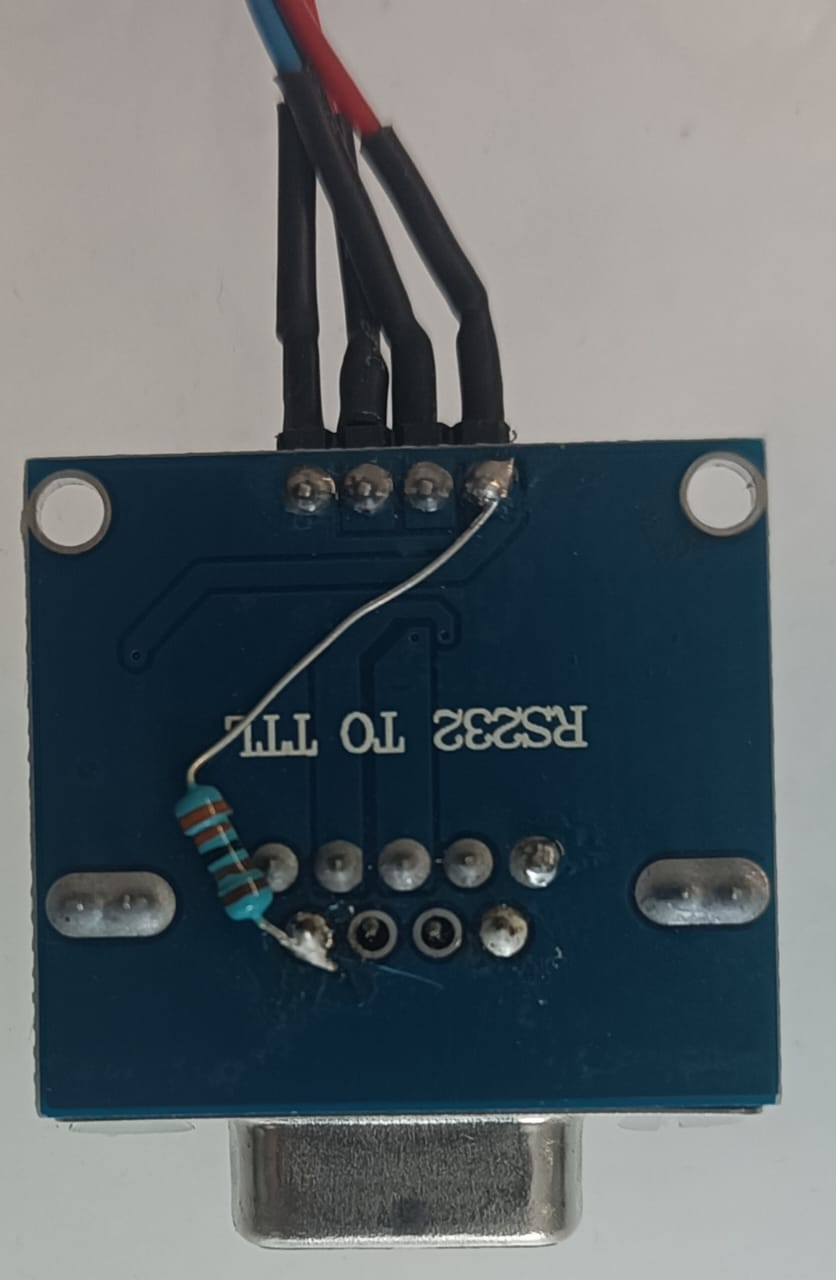
\includegraphics[angle=90, width=0.5\textwidth]{img/RS232_connector.jpeg}
          \caption{Picture of MAX3232 with 3.5kOhm pull-up resistor.}
          \label{MAX3232}
    \end{figure}

Some code that successfully enables communication between an Arduino DUE and the multimeter can be found in the project under Code that worked. This is useful to test initial communication with the multimeter. The connections of the Arduino DUE and the MAX3232 module are as shown in Figure \ref{MAX3232_Arduino}.

\begin{figure}[H]
          \centering
          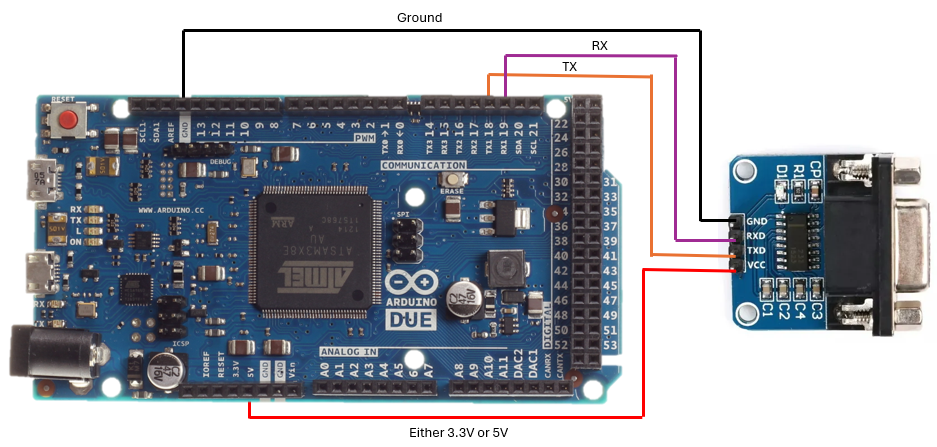
\includegraphics[width=1\linewidth]{img/MAX3232_connection.png}
          \caption{Electrical connection of Arduino DUE and MAX3232.}
          \label{MAX3232_Arduino}
    \end{figure}


\subsection{PCB version 1}
After some prototyping with a breadboard, the first version of the PCB was developed. It was given the name 'Automated DMM tester V1'. The purpose of this version is to test everything works smoothly and identify areas of improvement. 

A 16 channel MUX was chosen to direct the current of each ePATH pin to the multimeter so that the tests can be performed. A MUX was chosen over alternatives, such as shift registers with relays, for its simple wiring and fast operation \cite{tiMAX3232guide}. A 16 channeled one was chosen as there are 12 pins to be tested.

The kiCAD design of the PCB is stored in the project as PCB attempt 1. When soldering the components on the board some alternations were made; instead of $330\,\Omega$ resistors, $1.6k\,\Omega$ resistors were used and instead of $10k\,\Omega$ resistors $4.6k\,\Omega$ resistors were used. The Arduino program used on it to test the functionality of the board is saved in the project as PCB programming. 

In the schematic, the $330\,\Omega$ resistors were chosen since the forward voltage drop for white LEDs is approximately 2.4V and the desired current flow through them is about 10mA. Therefore:
\[
R = \frac{V}{I} = \frac{5\,\mathrm{V} - 2.4\,\mathrm{V}}{10\,\mathrm{mA}}=260\Omega
\]
Since $330\,\Omega$ is very close to the desired resistance and is a more readily available resistor value it was chosen.


There was a number of errors with this design:
\begin{itemize}
\item The symbol used for the banana socket is wrong. It represents the banana socket as a one-pin connector but it has 4 connecting terminals. This led to receiving an inquiry about it from the manufacturers.
\item The orientation of the button footprint is incorrect-it should be rotated by 90 degrees. This issue was bypassed when making the button connection to the board but an awkward connection was produced.
\item When testing with the ePATH board it was discovered that upon trying to measure negative voltages with the board the circuit stopped working. Upon testing the board, it was established that it can mesure a minimum of around -0.5V. Therefore, a different MUX or a different design should be used.
\item The wiring of the Restart button is incorrect. It was not connected to the Arduino DUE pin 8 properly. This was corrected on the board by adding a wire according to the diagram in Figure \ref{button_wiring}.
\end{itemize}

\begin{figure}[H]
          \centering
          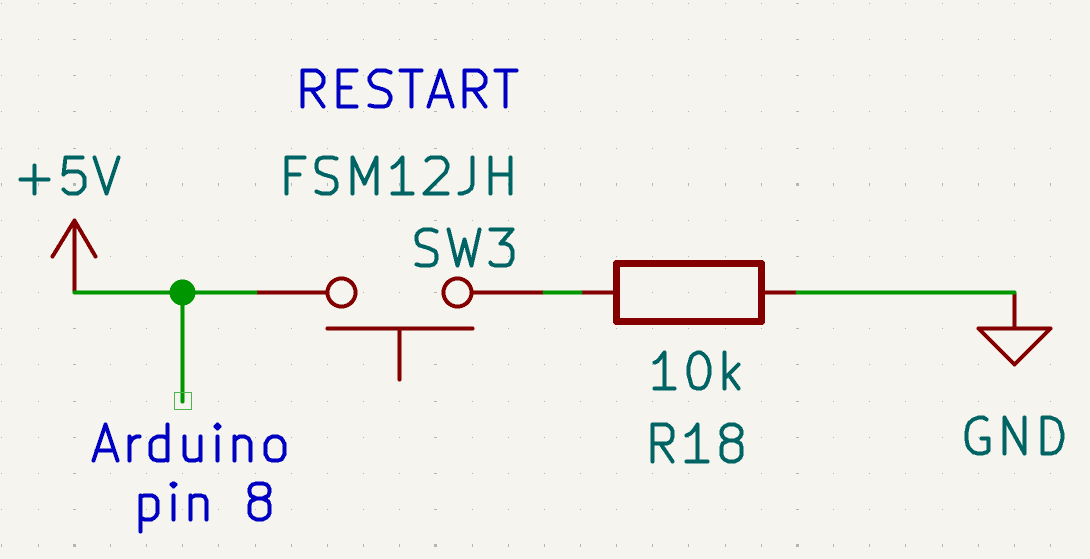
\includegraphics[width=1\linewidth]{img/button_wiring.png}
          \caption{Corrected electrical connection of RESTART button}
          \label{button_wiring}
    \end{figure}



\subsection{PCB version 2}
The improvements made for the second version of the PCB include:
\begin{itemize}
\item Some different electrical components were chosen, such as the MUX, that were more appropriate for the last scale production of the custom PCB board.
\item Implemented the PN532 module capable of obtaining the RFID tag of the ePATH board \cite{pn532manual}.
\item Implement a connector to enable easy connection of custom PCB with ePATH PCB.
\item l
\end{itemize}




\subsection{GUI}
A user friendly GUI has been developed to facilitate the testing of the ePATH PCB. The code for the GUI is on the ePATH-Test-Bench project of the company's GitHub \href{https://github.com/pathfinder-medical/ePATH-Test-Bench}{here}.

The key functionalities of the GUI include:
\begin{itemize}
\item Run button; Starts the testing cycle.
\item Clear button; Deletes all testing results for re-tests.
\item Save button; Saves a pdf file with the table of results.
\item Get button; Gets the RFID of the ePATH board.
\end{itemize}

\section{Results}

\subsection{Subtopic}
\lipsum[2]

\begin{table*}[ht]
    \centering
    \begin{tabular}{p{0.25\linewidth}p{0.25\linewidth}p{0.25\linewidth}}
    \hline
    column 1 & column 2 & column 3\\
    \hline
    1 & 2 & 3\\
    1 & 2 & 3\\
    1 & 2 & 3\\
    1 & 2 & 3\\
    \hline
    \end{tabular}
    \caption{Another random table}
    \label{tab:2}
\end{table*}
\noindent Another type of table for your results below.

\subsection{Subtopic 2}
\lipsum[1]

\noindent Another figure grid example: (on next page)

\begin{figure*}[ht]
\begin{multicols}{2}
        \centering
        \begin{subfigure}[b]{0.475\textwidth}
            \centering
            
\includegraphics[width=\textwidth]{img/bioeng.jpg}
            \caption{Part 1}    
        \end{subfigure}
        \hfill
        \begin{subfigure}[b]{0.475\textwidth}  
            \centering 
            
\includegraphics[width=\textwidth]{img/bioeng.jpg}
            \caption{Part 2}    
        \end{subfigure}
        \vskip\baselineskip
        \begin{subfigure}[b]{0.475\textwidth}   
            \centering 
            
\includegraphics[width=\textwidth]{img/bioeng.jpg}
            \caption{Part 3}  
        \end{subfigure}
        \hfill
        \begin{subfigure}[b]{0.475\textwidth}   
            \centering 
            
\includegraphics[width=\textwidth]{img/bioeng.jpg}
            \caption{Part 4}    
        \end{subfigure}
        \label{fig:mean and std of nets}
        \end{multicols}
        \caption {A figure grid} 
        \label{fig:3}
    \end{figure*}

\section{Discussion}

\subsection{Subtopic}
\lipsum[1]
\subsubsection{Part 1}
\lipsum[1]
\section{Conclusion}

\subsection{Summary}
\lipsum[2]

\noindent If you want to list some of your closing points here is an example:
Our concluding points are...
\begin{enumerate}
  \item Concluding point .....
  \item Concluding point.....
  \item Concluding point.....
\end{enumerate}


\subsection{Future Work}

\noindent To close this template, let's look at referencing. Make sure you have a references.bib files (check the example in this template) and then cite as follows:

\noindent Here I am mentioning something linked to my first reference. \cite{Barbero2012} 

\noindent Here I am mentioning something linked to my second reference. \cite{Farina2020}

\noindent Here I am mentioning something linked to my third reference. \cite{Saitou2000}

\noindent Make sure to check the latex documentation to reference different types of resources e.g. books, general communication, conference poster etc. in the correct way.

\newpage

\section{Appendix}

\noindent Add supplementary project information here. DON'T use as a workaround for the word count!!!
\bibliographystyle{plain}
\bibliography{references}

\end{document}